%%%%%%%%%%%%%%%%%%%%%%%%%%%%%%%%%%%%%%%%%
% fphw Assignment
% LaTeX Template
% Version 1.0 (27/04/2019)
%
% This template originates from:
% https://www.LaTeXTemplates.com
%
% Authors:
% Class by Felipe Portales-Oliva (f.portales.oliva@gmail.com) with template 
% content and modifications by Vel (vel@LaTeXTemplates.com)
%
% Template (this file) License:
% CC BY-NC-SA 3.0 (http://creativecommons.org/licenses/by-nc-sa/3.0/)
%
%%%%%%%%%%%%%%%%%%%%%%%%%%%%%%%%%%%%%%%%%

%----------------------------------------------------------------------------------------
%	PACKAGES AND OTHER DOCUMENT CONFIGURATIONS
%----------------------------------------------------------------------------------------

\documentclass[
	12pt, % Default font size, values between 10pt-12pt are allowed
	%letterpaper, % Uncomment for US letter paper size
	%spanish, % Uncomment for Spanish
]{fphw}

% Template-specific packages
\usepackage[utf8]{inputenc} % Required for inputting international characters
\usepackage[T1]{fontenc} % Output font encoding for international characters
\usepackage{mathpazo} % Use the Palatino font
\usepackage[dvipsnames]{xcolor}
\usepackage{graphicx} % Required for including images
\usepackage{amsmath}
\usepackage{booktabs} % Required for better horizontal rules in tables
\usepackage{listings} % Required for insertion of code
\usepackage{enumerate} % To modify the enumerate environment
\usepackage{ragged2e}
\usepackage{cancel}
\usepackage{MnSymbol,bbding,pifont}
\usepackage{lscape}
\usepackage{array}
\usepackage{float,graphicx}
\usepackage{hyperref}
\newcolumntype{M}{>{$}c<{$}}
%----------------------------------------------------------------------------------------
%	ASSIGNMENT INFORMATION
%----------------------------------------------------------------------------------------

\title{Assignment \#1} % Assignment title

\author{Luis Alberto Ballado Aradias} % Student name

\date{\today} % Due date

\institute{Centro de Investigación y de Estudios Avanzados del IPN \\ Unidad Tamaulipas} % Institute or school name

\class{CONTROL AUTOMÁTICO (Sep - Dec 2022)} % Course or class name

\professor{Dr. José Gabriel Ramírez Torres} % Professor or teacher in charge of the assignment

%----------------------------------------------------------------------------------------

\begin{document}

\maketitle % Output the assignment title, created automatically using the information in the custom commands above

%----------------------------------------------------------------------------------------
%	ASSIGNMENT CONTENT
%----------------------------------------------------------------------------------------
\section*{{\color{Apricot}Climate-neutral container terminal: How does it work?} \url{https://www.youtube.com/watch?v=wiKS-RYf-cY}}

La automatización en puertos maritimos ha tomado un auge de la mano con la industria 4.0 y la era del internet, la automatización como el uso de energia verdes nos comienza a acompañar a donde sea que vayamos. La globalización se ha convertido en una tendencia en la economía global y los sistemas de control automáticos son una pieza clave.\\

\begin{figure}[H]
  \centering
  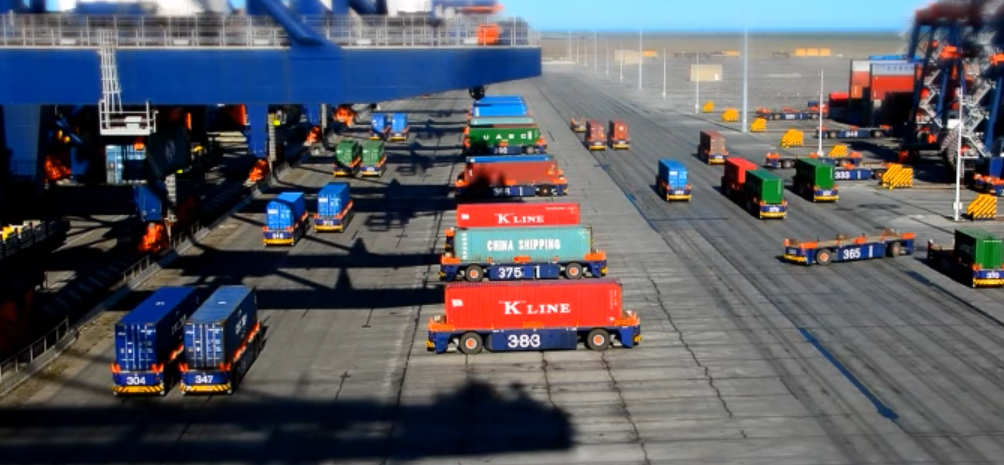
\includegraphics[scale=0.4]{images/agv.png}
\end{figure}

Según los datos de las \href{https://news.un.org/es/story/2021/11/1500122}{Naciones Unidas} el embate provocado por la pandemia de COVID-19 sobre el transporte maritimo de mercancias tuvo menos repercusión ya que la demanda global ocacionada por las compras electrónicas ayudo en generar un aumento del 4,3\% en 2021. \\

Para cualquier empresa donde las tareas se convierten en repetitivas y aburridas, es de buena opción automatizar dichos procesos cuando estos sean tecnológicamente posibles, ya que tareas comunes como cocinar, hacer una limpieza en áreas con muchos objetos suelen ser dificiles de automatizar.\\

\begin{figure}[H]
  \centering
  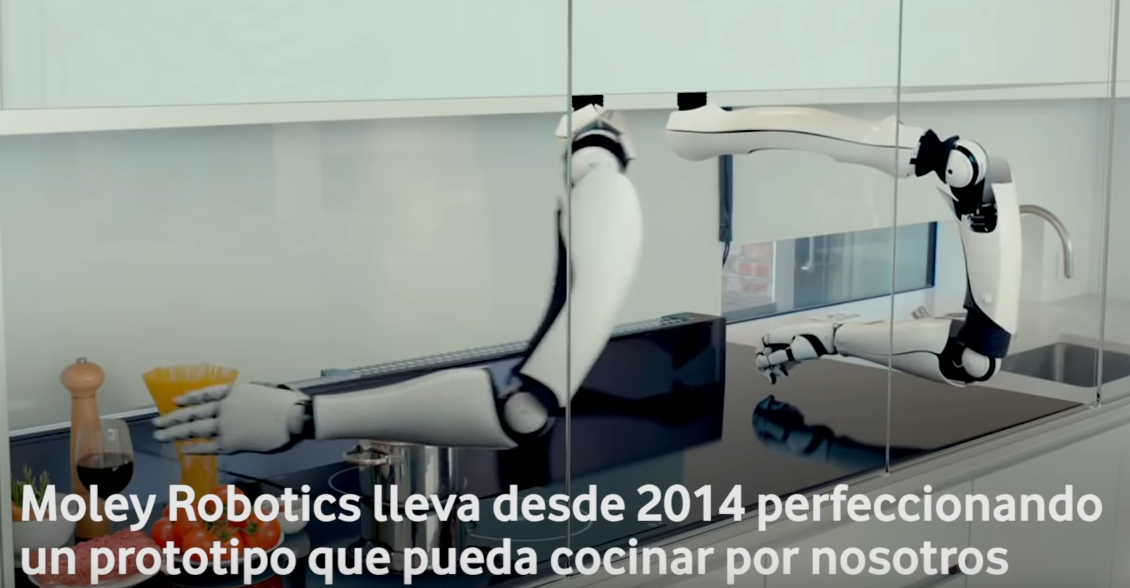
\includegraphics[scale=0.4]{images/hard.png}
\end{figure}

El futuro de la logistica, transporte marítimo ó terrestre tiene un futuro inteligente y sostenible. Teniendo ejemplos tangibles en los Puertos de Hamburgo, Shangai, Rotterdam por mencionar algunos.\\

La implementacion de vehículos AGV (Automated Guided Vehicles) en la industria de la logistica ha tomado un gran auge, no es dificil pensar que el grande de las ventas por internet AMAZON tenga una implementación en sus centros de distribución de ultima milla casi todo automatizado.\\

Para su construcción, mantenimiento, y desarrollo de sistemas inteligentes es de suma importancia el estudio de Sistemas de Control.

\newpage
\section*{{\color{Apricot}Why learn control systems at all?} \url{https://www.youtube.com/watch?v=oBc_BHxw78s}}

Los sistemas de control son la pieza que une todos los campos de la ingenieria.\\

Considerando algunos campos de la ingenieria podemos entender un poco más la importancia en el estudio del Control automático.

\begin{itemize}
\item Ingenieria Eléctica, en el diseño de reguladores y retroalimentaciones.
\item Ingenieria en Comunicaciones, en el diseño de controles de ganancia automáticas que incrementen la ganancia en señales débiles o decrementarlas en señales fuertes.
\item Ingeniera Mecánica, en la consideración de vibraciones, diseño de sistemas que aislen las vibraciones. 
\item Ingeniera Civil, en el diseño de construcciones resistentes a actividades sismicas.
\item Ingeniera Industrial, en el diseño de robótica para lineas de ensamblaje o diseño de controles PID para aplicaciones en la robótica.
\item Ingeniera Aeroespacial, en la creación de sistemas aerodinamicos resistentes a las vibraciones.
\end{itemize}

Esas se pueden tomar como ejemplos en donde los \textbf{sistemas de control} toman un papel importante. Una perspectiva general de los sistemas de control sería cuando se nos cae un objeto, éste vibrará y generará un sonido que se reducira a medida que la energía se disipe, o cuando intentamos detener una caida de algun objeto y este cae, causamos una disipasión rápida de la energía. \\

Una copa de vino cayendo se puede interpretar como la tecnologia detrás de un giroscopio (se basa en una masa girando sobre un eje, la cual se mantiene estable por el momento de rotación que tiene la masa), tecnologia usada en submarinos y satelites para una navegación por estima (inferir la ubicación haciendo uso de fórmulas trigonométricas)\\

\textbf{Teoria de Sistemas de Control} es más que adecuar un control PID y pendulos invertidos. Es contruir modelos de sistemas y poder simularlos para hacer predicciones y de esa forma entender la dinamica y como interactua con el resto del sistema.

\begin{itemize}
\item Es filtrar ruido y reducir las perturbaciones
\item Es diseñar o elegir los sensores o actuadores adecuados
\item Es probar los sistemas para asegurar que funcionará de manera adecuada en situaciones no pensadas
\item Es entender los sistemas en un nivel muy básico.
\end{itemize}

\newpage
\section*{{\color{Cerulean} Automation} \url{https://www.youtube.com/watch?v=XJLMW6l303g}}

\begin{figure}[H]
  \centering
  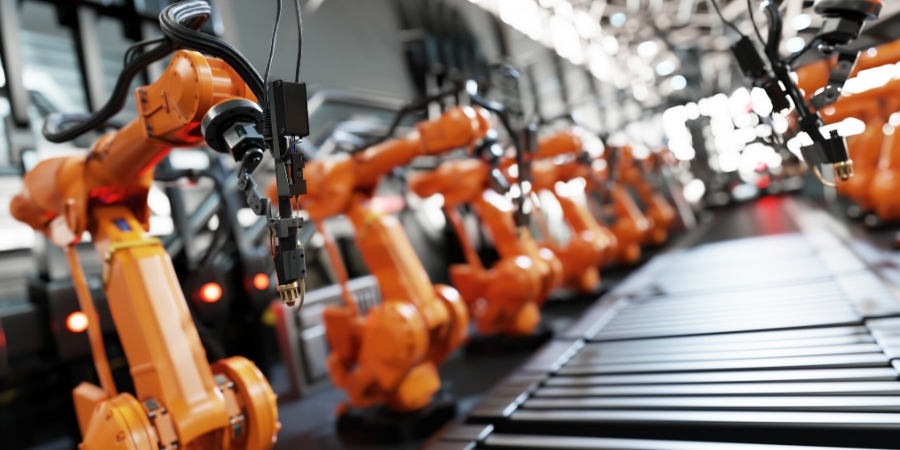
\includegraphics[scale=0.3]{images/automation.jpg}
\end{figure}


\textbf{Automatización} es una palabra que se ha tomado milenios en ser formada intervenida, convinando arte e ingenio, pero la ciencia detras tiene menos de dos milenios, pero la palabra automatización unas pocas decadas. No es dificil recordar los dispositivos autómatas en la historia, cuando se creaban artefactos para realizar tareas comunes. No todos los artefactos tenían el mismo uso, en ocaciones solo servian para entretener y no hacian nada mas que los mismos movimientos una y otra vez.

\begin{figure}[H]
  \centering
  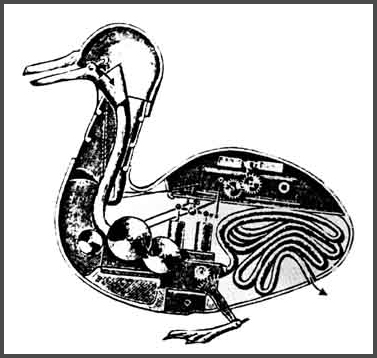
\includegraphics[scale=0.6]{images/pato.jpg}
  \caption{Pato de Vaucanson}
\end{figure}

La \textbf{Automatización} se ocupa de las complejas actividades que se necesitan ser resumidas en desiciones racionales y consisas, confiando en la información disponible y en las matemáticas. Pero básicamente la automatización es el desarrollar tareas de una manera automática.\\

En un vista general se comienza con la representación del sistema que se se desea controlar, linelizarlo, analizar su respuesta al impulso, aplicarle la transformada de LaPlace para pasarlo del dominio de la frecuencia y hacer un sin fin de calculos que nos ayudan a completar el objetivo de automatizar y controlar nuestro sistema. \\

Sea a lo que nos enfrentemos necesitaremos tres elementos fundamentales:

\begin{itemize}
\item Retroalimentación, que nos indique como van las cosas.
\item Control, la inteligencia que apartir de las retroalimentaciones decida que acción hacer. 
\item Actuador, la manera en que ejecutamos la acción.
\end{itemize}

Un ejemplo básico para el entendimiento de estos elementos es el cepillado de dientes. Al tener una retroalimentación de la posición del cepillo de dientes es fácil controlar la posición y el desplazamiento para las siguientes posiciones que requerimos para limpiar nuestros dientes. Pero, ¿qué pasaría sin alguno de estos tres elementos?

\begin{itemize}
\item Sin retroalimentación, no podríamos conocer la posición del cepillo y no podríamos indicar la siguiente posición. 
\item Sin Control, no podríamos saber que hacer ni como hacerlo  
\item Sin Actuador, no podríamos realizar el cepillado 
\end{itemize}

\begin{figure}[H]
  \centering
  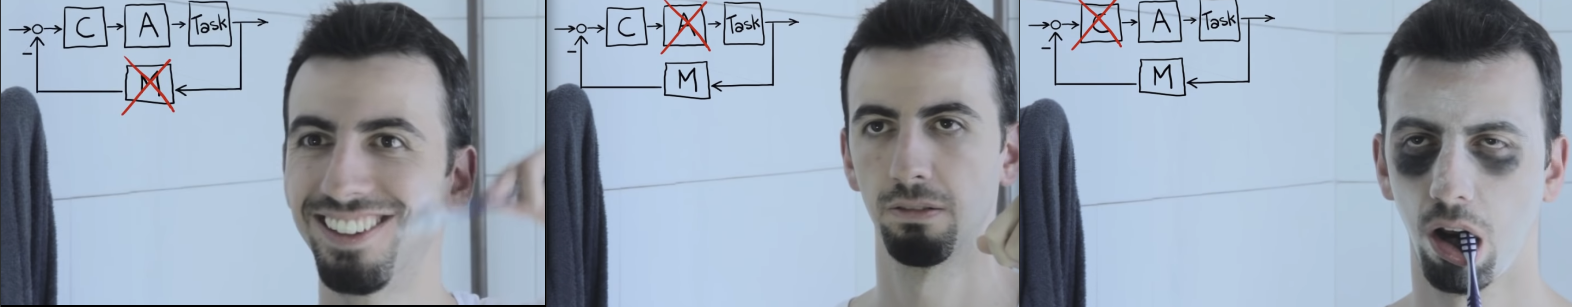
\includegraphics[scale=0.3]{images/ejemplo_control.png}
  \caption{Ejemplos sin algun elemento de control}
\end{figure}

Bajo éste ejemplo hemos visto el rol importante de cada elemento que forma parte de un sistema, ya que son importantes para realizar cualquier tarea.

\newpage
\section*{{\color{RoyalPurple}Tacoma Bridge} \url{https://www.youtube.com/watch?v=3mclp9QmCGs}}

El puente de Tacoma, fué construido en 1940 durando solamente 4 meses antes de su colapso en Noviembre 7 de 1940.\\

Apesar de las vibraciones que se observaron en su construcción, pero ese día la resonancia del puente y su movimiento de torsión debido a vientos más rápidos (65km/h) hizo que su movimiento natural de oscilación tuviera un periodo de 5 segundos.\\

La caída fué debido al fenómeno de resonancia mecánica que se poduce cuando un cuerpo que puede vibrar es sometido a una acción periódica y cuyo período coincide con el período del propio cuerpo causando que el cuerpo vibre aumentando su amplitud. 

\begin{figure}[H]
  \centering
  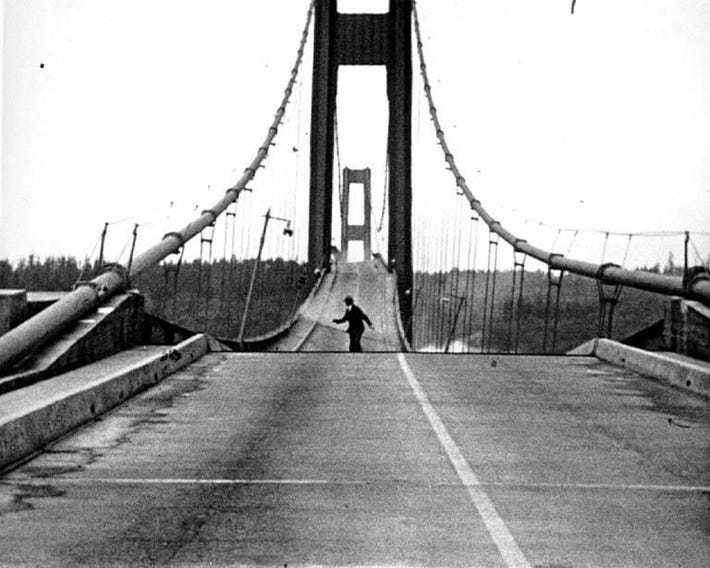
\includegraphics[scale=0.4]{images/tacoma.jpg}
\end{figure}

El desastre sirvió para la mejora de las nuevas construcciones de puentes colgantes en todo el mundo. El puente de tacoma fué reconstruido y reinagurado en 1950 y aún existe en nuestros días.

\newpage
\section*{{\color{RoyalPurple}What Control Systems Engineers Do?} \url{https://www.youtube.com/watch?v=ApMz1-MK9IQ}}

Ser un Ingeniero de Sistemas de Control es más que diseñar controles y adecuarlos. Puede que en el transcurso de un proyecto, el diseño del controlador sea una parte pequeña del trabajo. 
\begin{itemize}

\item \textbf{Formulacion/Requisitos}, antes de que tengamos idea de lo que se desea construir, la fase de formulación es donde se intenta descubrir la necesidad; dicha necesidad puede provenir de un cliente o un miembro de la empresa que cree que existe un mercado para un determinado producto. El equipo comercial sabe que se puede vender, pero no sabe cual es la mejor manera de hacerlo ni las dificultades técnicas para realizarlo. Como Ingeniero de Sistemas de Control una de las tareas es explorar desde una perspectiva ingenieril y buscar cual es la mejor opción. \\
Después de todo esto, es imposible conocer la configuración final que el usuario tendrá operando nuestros productos, de esa maneara hay que estar seguros que cuando el sistema este en uso la incertidumbre sea algo que cumpla con los requisitos y visualizar todos los posibles errores es factor para que los costos del producto se mantengan bajos. A menudo se suele listar las restricciones del sistema, presupuestos técnicos y bocetos del producto esperado y el equipo de ingenieria es el responsable de crear y administrar estos documentos.

\item \textbf{Desarrollo}, con las definiciones y requerimientos completos el desarrollo del producto puede comenzar. Esta fase describe el cliché de un ingeniero: Diseña cosas, construye cosas y prueba cosas. Esta fase de desarrollo suele tener correcciones y sufrir cambios. Supongamos que ya tenemos pensado el control que queremos aplicar, pero en las pruebas su tiempo de respuesta no es el esperado por los clientes en conclusión, se tendrá que modificar y probar nuevamente los test que ya fueron aplicados.\\

  Ya que los cambios son inevitables se tomará mucho tiempo en la etapa de desarrollo. En algunas compañias el Ingeniero de Control es el reponsable de crear y describir algoritmos y logica para las leyes de control en una forma que los Ingenieros de Software puedan entender y codificar.
  
\item \textbf{Pruebas/Verificaciones}, existen diferentes métodos de verificación y como Ingeniero en Control se deben de emplear algun método existente para la verificación del producto. Supongamos que deseamos probar un equipo físico, esto puede llevar mucho tiempo ya que no es lo mismo que simplemente correr un simulador. Hay que escribir un plan para desarrollar las pruebas, documentación de las pruebas. \\

  Para el final de la fase de Ingenieria se tendrá un diseño que cumple con las solicitudes planteadas al principio. Sin embargo el trabajo del Ingeniero de Control no termina ahí, es posible que sea requerido para capacitar los operadores del sistema o cubrir alguna variante del diseño o modificaciones en el vuelo. Los Sistemas de Control tienen muchas oportunidades en todas las fases del producto y no es tarea de una sola persona, se requiere el trabajo en equipo.
  
\end{itemize}
\newpage
\section*{{\color{RoyalPurple}Control Systems Lectures LTI Systems} \url{https://www.youtube.com/watch?v=3eDDTFcSC_Y}}

Los sistemas lineales e invariantes en el tiempo (LTI) son una clase de sistemas que responden de una determinada manera cuando se le aplica una entrada arbitraria, todos los sistemas LTI tienen propiedades en común
\begin{itemize}
\item \textbf{Homogeniedad}, supongamos que tenemos un sistema LTI y le inyectamos una entrada $x(t)$, esta producirá una salida $y(t)$. La Homogeniedad nos dice que si escalamos la entrada en un factor, entonces el resultado será escalado con el mismo factor 
\item \textbf{Superposición (Aditividad)}, digamos añadimos dos entradas juntas $x_{1} + x_{2}$, el resultado será la superposición de las dos salidas. Algunas veces la homogeniedad y susperposición son combinadas para que cuando la entrada sea escalada y sumada por la misma cantidad, si el sistema conoce estos dos criterios, se llamará un sistema lineal.
\item \textbf{Invarianza de Tiempo}, por ejemplo si dejamos caer un objeto por las escaleras, este tendrá el mismo comportamiento independientemente que hora del día sea. En otras palabras, una entrada $x(t-a)$ producirá una salida $y(t-a)$ es decir, dos entradas similares en el transladadas en el tiempo tendrán la misma salida. Este termino de Invarianza de tiempo se puede referir de un termino más generico llamado \textbf{traslación invariante}, que también se puede decir como \textbf{traslación en el espacio}
\end{itemize}

Estas tres restricciones son las que se necesitan para tener un sistema LTI, pero ¿por qué son importantes los sistemas LTI?- Richard Feynman dicia que son importantes ya que los podemos resolver. Ya que los sistemas físicos se pueden aproximar con modelos LTI.\\

Los sistemas LTI se caracterisan en la respuesta al impulso, por ejemplo si golpeamos un objeto este se moverá y después de un tiempo dejará de hacerlo. Debido al principio de invariante en el tiempo si golpeamos el objeto en un tiempo 0, y continuamos haciendolo en el tiempo 1 podemos esperar el mismo comportamiento y por la característica de homogeniedad, si lo golpeamos con más fuerte esperaremos una respuesta más larga y por la característica de superposición, la respuesta completa del sistema será la sumatoria total de las señales. Podemos hacer que nuestro sistema se aproxime a la linealidad con la sumatoria de todas las señales individuales.\\

Cuando hacemos la sumatoria en el dominio del tiempo es llamada \textbf{convolución}, que puede ser una Integral difícil de resolver, sin embargo transformamos las respuestas al impulso y las entradas del sistema al dominio $S$ usando la transformada de Laplace, entonces la \textbf{convolución} se convierte en una multiplicación algebraica. Esto solo aplica a los sistemas LTI.

\newpage
\section*{{\color{RoyalPurple}Laplace transform} \url{https://www.youtube.com/watch?v=VJ9phDRys_I}}

La Transformada de Laplace es de ayuda para entender las funciones de transferencia. Una forma sencilla de entender la transformada de Laplace es haciendo un contraste con la Transformada de Fourier. Una Transformada de Fourier mapea una señal del dominio del tiempo al dominio de la frecuencia el cual es una función de dos dimensiones (Una dimensión para la magnitud y otra dimensión para la fase), mientras la transformada de Laplace al dominio de $s$.

Como ejemplo en una caida exponencial, cuyo valor es 0 para todos los valores en tiempo negativo, la ecuación para está función es $u(t)$, que es solamente la función escalón multiplicado por $e^{-t}$.

\begin{figure}[H]
  \centering
  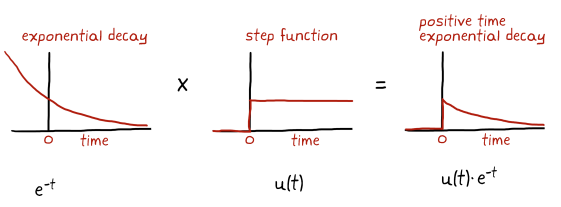
\includegraphics[scale=0.6]{images/decay_function.png}
\end{figure}

La Transformada de Fourier para $f(t)=u(t)*e^{-t}$ puede ser representada como: $\frac{1}{1+jw}$, notemos que el resultado es una función compleja ya que la variable imaginaria $j$ esta dividida por $1+jw$, ahora por definición las funciones de dos dimensiones estan formadas de una parte real y una parte imaginaria. Podemos decir que la ecuación tiene dos componentes real: $\frac{1}{1+w^{2}}$ e imaginaria: $-j\frac{w}{1+w^{2}}$ \\

En este punto, calcular la magnitud y la fase es convertirlo a una representación de coordenadas rectangulares, las cuales son las partes reales e imaginarias a coordenadas polares.

\begin{figure}[H]
  \centering
  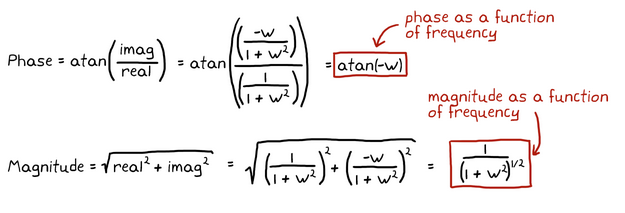
\includegraphics[scale=0.4]{images/funciones.png}
\end{figure}

Ahora podemos tener un panorama a partir de un decaimiento de una función exponencial en el tiempo y terminando con dos dimensiones magnitud y fase en función de omega, donde omega describe el valor de la frecuencia. A medida que avanzamos hacia el plano S. La transformada de Laplace va un paso más allá de la transformada de Fourier que ademas de descomponer la señal en ondas de coseno y funciones exponenciales, la transformada de Laplace necesita una variable que pueda tener esos conceptos y es ahí donde entra $S$ que es una variable compleja por lo que es bidimensional y contiene información de frecuencia $jw$.\\

Podemos reemplazar los coeficientes de $t$ en el exponente con la variable $\sigma$, teniendo como resultado $f(\sigma)=e^{\sigma t}$

Diferencias entre la Transformada de Fourier vs Transformada de Laplace
\begin{figure}[H]
  \centering
  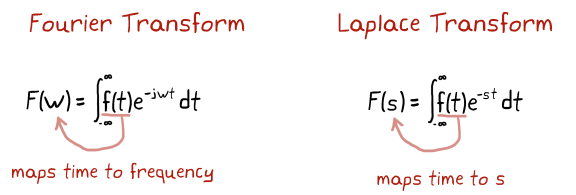
\includegraphics[scale=0.5]{images/fourier_laplace.png}
\end{figure}

La transformada de fourier solo es para funciones definidas para todos los números reales, sin embargo la transformada de laplace no requiere la función definida en el conjunto de los números reales negativos. La transformada de fourier es un caso especial de la transformada de Laplace. Cada función que tiene transformada de fourier tendrá su transformada de Laplace, pero no al revés.

\begin{figure}[H]
  \centering
  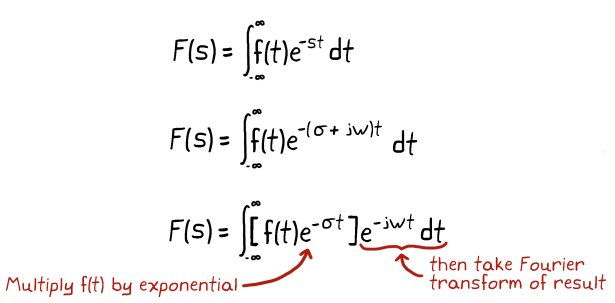
\includegraphics[scale=0.5]{images/multiply.png}
\end{figure}

Si reemplazamos $s$ con $\sigma +  j\omega$ en la transformada de Laplace y luego reordenamos la ecuaci{on, encontramos que esencialmente la transformada de Laplace esta tomando la función original del tiempo multiplicado por una función exponencial y tomando la transformada de fourier como resultado.  

\newpage
\section*{{\color{RoyalPurple}Transfer functions} \url{https://www.youtube.com/watch?v=RJleGwXorUk}}

Las funciones de transferencia son la transformada de Laplace de una respuesta al impulso de un sistema LTI cuando las condiciones iniciales son $0$. Pensemos la función de transferencia como una caja negra, que cuando le aplicamos una señal impulso podremos tener una señal modificada de salida si diseñamos la caja negra de manera correcta. \\

La \textbf{función de trnasferencia} P(s) de un sistema se define como el factor, en la ecuación de Y(s), que multiplica a la transformada de la entrada X(s). Se puede decir que las funciones de transferencia son expresiones algebraicas racionales. La función de transferencia de un sistema que incluye retardos de tiempo, contiene terminos de la forma $e^{-st}$. De hecho, la función de transferencia de un elemento que representa un retardo de tiempo puro es $P(s) =e^{-sT}$ donde T es el retardo de tiempo en unidades de tiempo. \\

Puesto que la transformada de la salida Y(s) se forma simplemente con una multiplicación algebraica de P(s) y X(s) cuando es igual a 0, la multiplicación es conmutativa, es decir
\[Y(s)=X(s)P(s) = P(s)X(s)\]

Propiedades de una función de transferencia.

\begin{itemize}
\item La función de transferencia de un sistema es la transformada de Laplace de su respuesta al impulso. Es decir, si la entrada de un sistema con una función de transferencia P(s) es un impulso, y todos los valores iniciales son cero, la transformada de la salida es P(s).
\item La función de transferencia del sistema se puede determinar a partir de la ecuación diferencial del sistema, usando la transformada de Laplace e ignorando todos los términos ocasionados por valores iniciales. La función de transferencia P(s) está dada entonces por \[P(s)=\frac{Y(s)}{X(s)}\]

\item La ecuación diferencial del sistema se puede obtener de la función de transferencia remplazando la variable s por el operador diferencial D definido por $D=\frac{d}{dt}$ 
\item La estabilidad de un sistema lineal invariable con el tiempo se puede determinar de la ecuación característica. El denominador de la función de transferencia del sistema igualado a cero, constituye la ecuación caracteristica. En consecuencia, si todas las raíces del denominador tienen partes reales negativas, el sistema es estable.
\item Las raices del denominador son los polos del sistema y las raices del numerador son los ceros del sistema. La función de transferencia del sistema se puede especificar como una constante, especificando los polos y ceros del sistema. Esta constante, que generalmente se denota como K, es el \textbf{factor de ganancia} del sistema. 
\end{itemize}
\newpage
\section*{{\color{RoyalPurple}HOLA MUNDO en NXC}}

\begin{figure}[H]
  \centering
  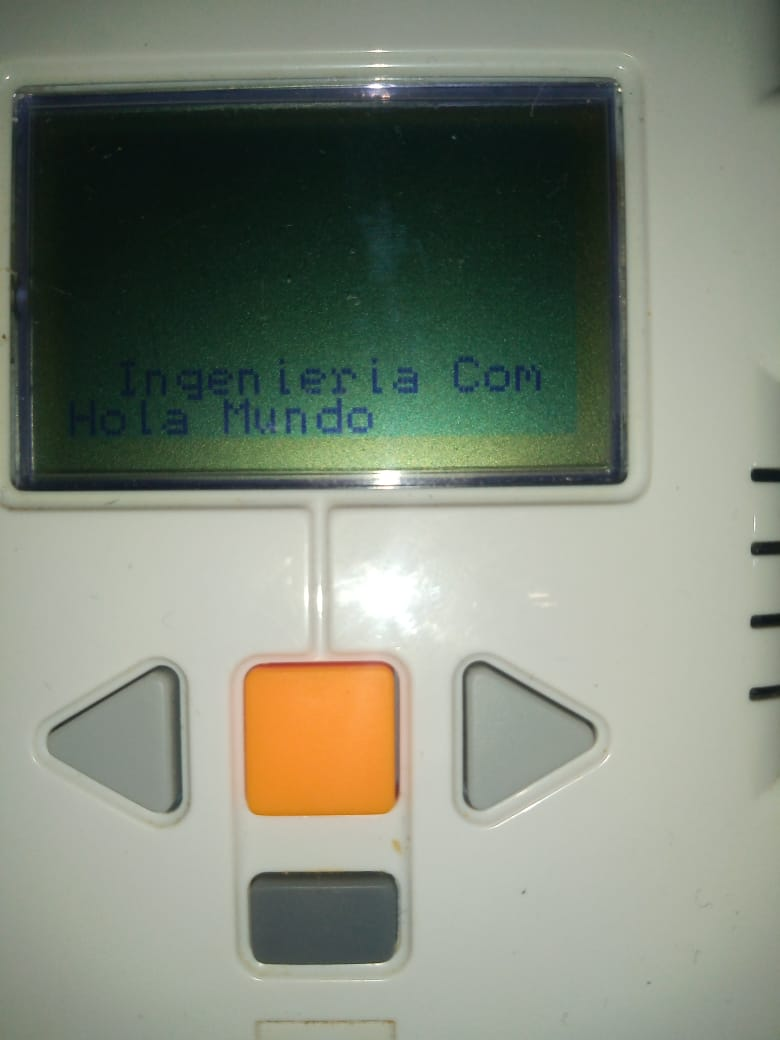
\includegraphics[scale=0.3]{images/luis_code.jpeg}
\end{figure}

\begin{verbatim}
task main()
{
  repeat(15000){
    TextOut(10,10,"Ingenieria Computacional");
    TextOut(1,1,"Hola Mundo");
  }
}
\end{verbatim}

A consecuencia que el proyecto NBC/NXC ya no ha tenido recientes actualizaciones, la instalación en una laptop con ubuntu 20.04 se llevó acabo con la siguiente adaptación.

\url{https://github.com/pierre-24/nbc-compiler}

De está forma se puede tener uso de los comandos de $nbc$ en las versiones recientes de linux. 

\end{document}
